% Genere par src/figures_generator/figures_composition.py. Ne pas editer a la main.
\definecolor{reltuned}{HTML}{0072B2}
\definecolor{relshelf}{HTML}{D55E00}
\begin{figure}[t]
\centering
% Options en clair plutot qu'un style nomme, pour la meme raison.
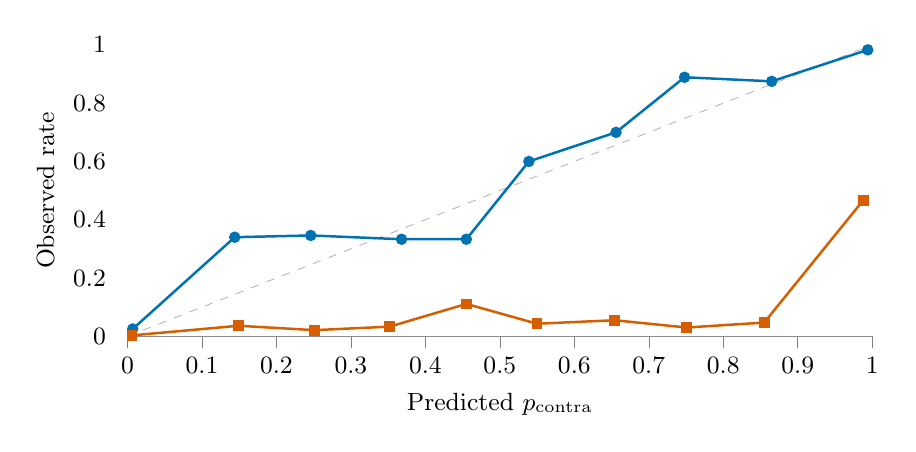
\begin{tikzpicture}
\begin{axis}[
  width=0.78\columnwidth, height=3.7cm, scale only axis,
  axis line style={draw=black!45, line width=0.3pt},
  axis x line*=bottom, axis y line*=left, y axis line style={draw=none},
  xmajorgrids=false, ymajorgrids=false, tick align=outside, ytick style={draw=none},
  xlabel={Predicted $p_{\mathrm{contra}}$}, ylabel={Observed rate},
  label style={font=\small}, tick label style={font=\small},
  xmin=0, xmax=1, ymin=0, ymax=1,
]
\addplot[draw=black!30, line width=0.3pt, dashed, mark=none, forget plot] coordinates {(0,0) (1,1)};
\addplot[draw=reltuned, line width=0.9pt, mark=*, mark size=1.6pt, mark options={draw=reltuned, fill=reltuned}] coordinates {(0.007,0.025) (0.144,0.340) (0.246,0.346) (0.368,0.333) (0.455,0.333) (0.539,0.600) (0.656,0.700) (0.748,0.889) (0.865,0.875) (0.994,0.983)};
\addplot[draw=relshelf, line width=0.9pt, mark=square*, mark size=1.5pt, mark options={draw=relshelf, fill=relshelf}] coordinates {(0.006,0.003) (0.149,0.036) (0.251,0.021) (0.352,0.033) (0.455,0.111) (0.550,0.043) (0.654,0.055) (0.751,0.030) (0.855,0.047) (0.988,0.467)};
\end{axis}
\end{tikzpicture}
\caption{Reliability of $p_{\mathrm{contra}}$, SICK test half, ten bins. The dashed diagonal is perfect calibration. The \textcolor{reltuned}{\textbf{fine-tuned head}} tracks it, the \textcolor{relshelf}{\textbf{off-the-shelf head}} falls far below.}
\label{fig:reliability}
\end{figure}
